% Options for packages loaded elsewhere
\PassOptionsToPackage{unicode}{hyperref}
\PassOptionsToPackage{hyphens}{url}
%
\documentclass[
]{article}
\usepackage{lmodern}
\usepackage{amssymb,amsmath}
\usepackage{ifxetex,ifluatex}
\ifnum 0\ifxetex 1\fi\ifluatex 1\fi=0 % if pdftex
  \usepackage[T1]{fontenc}
  \usepackage[utf8]{inputenc}
  \usepackage{textcomp} % provide euro and other symbols
\else % if luatex or xetex
  \usepackage{unicode-math}
  \defaultfontfeatures{Scale=MatchLowercase}
  \defaultfontfeatures[\rmfamily]{Ligatures=TeX,Scale=1}
\fi
% Use upquote if available, for straight quotes in verbatim environments
\IfFileExists{upquote.sty}{\usepackage{upquote}}{}
\IfFileExists{microtype.sty}{% use microtype if available
  \usepackage[]{microtype}
  \UseMicrotypeSet[protrusion]{basicmath} % disable protrusion for tt fonts
}{}
\makeatletter
\@ifundefined{KOMAClassName}{% if non-KOMA class
  \IfFileExists{parskip.sty}{%
    \usepackage{parskip}
  }{% else
    \setlength{\parindent}{0pt}
    \setlength{\parskip}{6pt plus 2pt minus 1pt}}
}{% if KOMA class
  \KOMAoptions{parskip=half}}
\makeatother
\usepackage{xcolor}
\IfFileExists{xurl.sty}{\usepackage{xurl}}{} % add URL line breaks if available
\IfFileExists{bookmark.sty}{\usepackage{bookmark}}{\usepackage{hyperref}}
\hypersetup{
  pdftitle={reproducable research project 2},
  pdfauthor={Yaswanth Pulavarthi},
  hidelinks,
  pdfcreator={LaTeX via pandoc}}
\urlstyle{same} % disable monospaced font for URLs
\usepackage[margin=1in]{geometry}
\usepackage{color}
\usepackage{fancyvrb}
\newcommand{\VerbBar}{|}
\newcommand{\VERB}{\Verb[commandchars=\\\{\}]}
\DefineVerbatimEnvironment{Highlighting}{Verbatim}{commandchars=\\\{\}}
% Add ',fontsize=\small' for more characters per line
\usepackage{framed}
\definecolor{shadecolor}{RGB}{248,248,248}
\newenvironment{Shaded}{\begin{snugshade}}{\end{snugshade}}
\newcommand{\AlertTok}[1]{\textcolor[rgb]{0.94,0.16,0.16}{#1}}
\newcommand{\AnnotationTok}[1]{\textcolor[rgb]{0.56,0.35,0.01}{\textbf{\textit{#1}}}}
\newcommand{\AttributeTok}[1]{\textcolor[rgb]{0.77,0.63,0.00}{#1}}
\newcommand{\BaseNTok}[1]{\textcolor[rgb]{0.00,0.00,0.81}{#1}}
\newcommand{\BuiltInTok}[1]{#1}
\newcommand{\CharTok}[1]{\textcolor[rgb]{0.31,0.60,0.02}{#1}}
\newcommand{\CommentTok}[1]{\textcolor[rgb]{0.56,0.35,0.01}{\textit{#1}}}
\newcommand{\CommentVarTok}[1]{\textcolor[rgb]{0.56,0.35,0.01}{\textbf{\textit{#1}}}}
\newcommand{\ConstantTok}[1]{\textcolor[rgb]{0.00,0.00,0.00}{#1}}
\newcommand{\ControlFlowTok}[1]{\textcolor[rgb]{0.13,0.29,0.53}{\textbf{#1}}}
\newcommand{\DataTypeTok}[1]{\textcolor[rgb]{0.13,0.29,0.53}{#1}}
\newcommand{\DecValTok}[1]{\textcolor[rgb]{0.00,0.00,0.81}{#1}}
\newcommand{\DocumentationTok}[1]{\textcolor[rgb]{0.56,0.35,0.01}{\textbf{\textit{#1}}}}
\newcommand{\ErrorTok}[1]{\textcolor[rgb]{0.64,0.00,0.00}{\textbf{#1}}}
\newcommand{\ExtensionTok}[1]{#1}
\newcommand{\FloatTok}[1]{\textcolor[rgb]{0.00,0.00,0.81}{#1}}
\newcommand{\FunctionTok}[1]{\textcolor[rgb]{0.00,0.00,0.00}{#1}}
\newcommand{\ImportTok}[1]{#1}
\newcommand{\InformationTok}[1]{\textcolor[rgb]{0.56,0.35,0.01}{\textbf{\textit{#1}}}}
\newcommand{\KeywordTok}[1]{\textcolor[rgb]{0.13,0.29,0.53}{\textbf{#1}}}
\newcommand{\NormalTok}[1]{#1}
\newcommand{\OperatorTok}[1]{\textcolor[rgb]{0.81,0.36,0.00}{\textbf{#1}}}
\newcommand{\OtherTok}[1]{\textcolor[rgb]{0.56,0.35,0.01}{#1}}
\newcommand{\PreprocessorTok}[1]{\textcolor[rgb]{0.56,0.35,0.01}{\textit{#1}}}
\newcommand{\RegionMarkerTok}[1]{#1}
\newcommand{\SpecialCharTok}[1]{\textcolor[rgb]{0.00,0.00,0.00}{#1}}
\newcommand{\SpecialStringTok}[1]{\textcolor[rgb]{0.31,0.60,0.02}{#1}}
\newcommand{\StringTok}[1]{\textcolor[rgb]{0.31,0.60,0.02}{#1}}
\newcommand{\VariableTok}[1]{\textcolor[rgb]{0.00,0.00,0.00}{#1}}
\newcommand{\VerbatimStringTok}[1]{\textcolor[rgb]{0.31,0.60,0.02}{#1}}
\newcommand{\WarningTok}[1]{\textcolor[rgb]{0.56,0.35,0.01}{\textbf{\textit{#1}}}}
\usepackage{graphicx,grffile}
\makeatletter
\def\maxwidth{\ifdim\Gin@nat@width>\linewidth\linewidth\else\Gin@nat@width\fi}
\def\maxheight{\ifdim\Gin@nat@height>\textheight\textheight\else\Gin@nat@height\fi}
\makeatother
% Scale images if necessary, so that they will not overflow the page
% margins by default, and it is still possible to overwrite the defaults
% using explicit options in \includegraphics[width, height, ...]{}
\setkeys{Gin}{width=\maxwidth,height=\maxheight,keepaspectratio}
% Set default figure placement to htbp
\makeatletter
\def\fps@figure{htbp}
\makeatother
\setlength{\emergencystretch}{3em} % prevent overfull lines
\providecommand{\tightlist}{%
  \setlength{\itemsep}{0pt}\setlength{\parskip}{0pt}}
\setcounter{secnumdepth}{-\maxdimen} % remove section numbering

\title{reproducable research project 2}
\author{Yaswanth Pulavarthi}
\date{8/3/2020}

\begin{document}
\maketitle

\hypertarget{us-storm-data-analysis}{%
\section{US Storm data analysis}\label{us-storm-data-analysis}}

\hypertarget{data-processing}{%
\subsection{1 Data processing}\label{data-processing}}

loaded the data using read.csv function, because it can automatically
extracts file and load into csv. just took the required columns needed
for analysis and set cache= TRUE.

\hypertarget{load-data}{%
\subsection{load data}\label{load-data}}

\begin{Shaded}
\begin{Highlighting}[]
\KeywordTok{read.csv}\NormalTok{(}\StringTok{"C:}\CharTok{\textbackslash{}\textbackslash{}}\StringTok{Users}\CharTok{\textbackslash{}\textbackslash{}}\StringTok{Yaswanth Pulavarthi}\CharTok{\textbackslash{}\textbackslash{}}\StringTok{Downloads}\CharTok{\textbackslash{}\textbackslash{}}\StringTok{repdata_data_StormData.csv.bz2"}\NormalTok{)->data}
\KeywordTok{names}\NormalTok{(data)}
\end{Highlighting}
\end{Shaded}

\begin{verbatim}
##  [1] "STATE__"    "BGN_DATE"   "BGN_TIME"   "TIME_ZONE"  "COUNTY"    
##  [6] "COUNTYNAME" "STATE"      "EVTYPE"     "BGN_RANGE"  "BGN_AZI"   
## [11] "BGN_LOCATI" "END_DATE"   "END_TIME"   "COUNTY_END" "COUNTYENDN"
## [16] "END_RANGE"  "END_AZI"    "END_LOCATI" "LENGTH"     "WIDTH"     
## [21] "F"          "MAG"        "FATALITIES" "INJURIES"   "PROPDMG"   
## [26] "PROPDMGEXP" "CROPDMG"    "CROPDMGEXP" "WFO"        "STATEOFFIC"
## [31] "ZONENAMES"  "LATITUDE"   "LONGITUDE"  "LATITUDE_E" "LONGITUDE_"
## [36] "REMARKS"    "REFNUM"
\end{verbatim}

\begin{Shaded}
\begin{Highlighting}[]
\NormalTok{req.col<-}\KeywordTok{c}\NormalTok{(}\StringTok{"EVTYPE"}\NormalTok{,}\StringTok{"FATALITIES"}\NormalTok{,}\StringTok{"INJURIES"}\NormalTok{,}\StringTok{"PROPDMG"}\NormalTok{,}\StringTok{"PROPDMGEXP"}\NormalTok{,}\StringTok{"CROPDMG"}\NormalTok{,}\StringTok{"CROPDMGEXP"}\NormalTok{ )}
\NormalTok{data<-data[,req.col]}
\KeywordTok{head}\NormalTok{(data)}
\end{Highlighting}
\end{Shaded}

\begin{verbatim}
##    EVTYPE FATALITIES INJURIES PROPDMG PROPDMGEXP CROPDMG CROPDMGEXP
## 1 TORNADO          0       15    25.0          K       0           
## 2 TORNADO          0        0     2.5          K       0           
## 3 TORNADO          0        2    25.0          K       0           
## 4 TORNADO          0        2     2.5          K       0           
## 5 TORNADO          0        2     2.5          K       0           
## 6 TORNADO          0        6     2.5          K       0
\end{verbatim}

\hypertarget{damagecosts}{%
\subsection{damagecosts}\label{damagecosts}}

\hypertarget{property-damage-costs}{%
\subsubsection{property damage costs}\label{property-damage-costs}}

listed the types of property damage expenses using unique function

\begin{Shaded}
\begin{Highlighting}[]
\KeywordTok{unique}\NormalTok{(data}\OperatorTok{$}\NormalTok{PROPDMGEXP)}
\end{Highlighting}
\end{Shaded}

\begin{verbatim}
##  [1] "K" "M" ""  "B" "m" "+" "0" "5" "6" "?" "4" "2" "3" "h" "7" "H" "-" "1" "8"
\end{verbatim}

changed the character variables of PROPDMGEXP into numbers .i.e: K
=1000,M=1,000,000 and 0 for invalid data(?,+,-). And, created new colomn
in data table, which gives the information about property loss

\begin{Shaded}
\begin{Highlighting}[]
\CommentTok{# Assigning values for the property data }
\NormalTok{data}\OperatorTok{$}\NormalTok{PROPEXP[data}\OperatorTok{$}\NormalTok{PROPDMGEXP }\OperatorTok{==}\StringTok{ "K"} \OperatorTok{|}\StringTok{ }\NormalTok{data}\OperatorTok{$}\NormalTok{PROPDMGEXP }\OperatorTok{==}\StringTok{ "3"}\NormalTok{] <-}\StringTok{ }\DecValTok{1000}
\NormalTok{data}\OperatorTok{$}\NormalTok{PROPEXP[data}\OperatorTok{$}\NormalTok{PROPDMGEXP }\OperatorTok{==}\StringTok{ "M"} \OperatorTok{|}\StringTok{ }\NormalTok{data}\OperatorTok{$}\NormalTok{PROPDMGEXP }\OperatorTok{==}\StringTok{ "m"} \OperatorTok{|}\StringTok{ }\NormalTok{data}\OperatorTok{$}\NormalTok{PROPDMGEXP }\OperatorTok{==}\StringTok{ "6"}\NormalTok{] <-}\StringTok{ }\FloatTok{1e+06}
\NormalTok{data}\OperatorTok{$}\NormalTok{PROPEXP[data}\OperatorTok{$}\NormalTok{PROPDMGEXP }\OperatorTok{==}\StringTok{ ""}\NormalTok{] <-}\StringTok{ }\DecValTok{1}
\NormalTok{data}\OperatorTok{$}\NormalTok{PROPEXP[data}\OperatorTok{$}\NormalTok{PROPDMGEXP }\OperatorTok{==}\StringTok{ "B"}\NormalTok{] <-}\StringTok{ }\FloatTok{1e+09}
\NormalTok{data}\OperatorTok{$}\NormalTok{PROPEXP[data}\OperatorTok{$}\NormalTok{PROPDMGEXP }\OperatorTok{==}\StringTok{ "0"}\NormalTok{] <-}\StringTok{ }\DecValTok{1}
\NormalTok{data}\OperatorTok{$}\NormalTok{PROPEXP[data}\OperatorTok{$}\NormalTok{PROPDMGEXP }\OperatorTok{==}\StringTok{ "5"}\NormalTok{] <-}\StringTok{ }\FloatTok{1e+05}
\NormalTok{data}\OperatorTok{$}\NormalTok{PROPEXP[data}\OperatorTok{$}\NormalTok{PROPDMGEXP }\OperatorTok{==}\StringTok{ "4"}\NormalTok{] <-}\StringTok{ }\DecValTok{10000}
\NormalTok{data}\OperatorTok{$}\NormalTok{PROPEXP[data}\OperatorTok{$}\NormalTok{PROPDMGEXP }\OperatorTok{==}\StringTok{ "2"} \OperatorTok{|}\StringTok{ }\NormalTok{data}\OperatorTok{$}\NormalTok{PROPDMGEXP }\OperatorTok{==}\StringTok{ "h"} \OperatorTok{|}\StringTok{ }\NormalTok{data}\OperatorTok{$}\NormalTok{PROPDMGEXP }\OperatorTok{==}\StringTok{ "H"}\NormalTok{] <-}\StringTok{ }\DecValTok{100}
\NormalTok{data}\OperatorTok{$}\NormalTok{PROPEXP[data}\OperatorTok{$}\NormalTok{PROPDMGEXP }\OperatorTok{==}\StringTok{ "7"}\NormalTok{] <-}\StringTok{ }\FloatTok{1e+07}
\NormalTok{data}\OperatorTok{$}\NormalTok{PROPEXP[data}\OperatorTok{$}\NormalTok{PROPDMGEXP }\OperatorTok{==}\StringTok{ "1"}\NormalTok{] <-}\StringTok{ }\DecValTok{10}
\NormalTok{data}\OperatorTok{$}\NormalTok{PROPEXP[data}\OperatorTok{$}\NormalTok{PROPDMGEXP }\OperatorTok{==}\StringTok{ "8"}\NormalTok{] <-}\StringTok{ }\FloatTok{1e+08}
\CommentTok{# Assigning '0' to invalid data}
\NormalTok{data}\OperatorTok{$}\NormalTok{PROPEXP[data}\OperatorTok{$}\NormalTok{PROPDMGEXP }\OperatorTok{==}\StringTok{ "+"} \OperatorTok{|}\StringTok{ }\NormalTok{data}\OperatorTok{$}\NormalTok{PROPDMGEXP }\OperatorTok{==}\StringTok{ "-"} \OperatorTok{|}\NormalTok{data}\OperatorTok{$}\NormalTok{PROPDMGEXP }\OperatorTok{==}\StringTok{ "?"}\NormalTok{] <-}\StringTok{ }\DecValTok{0}
\CommentTok{# Calculating the property damage value}
\NormalTok{data}\OperatorTok{$}\NormalTok{PROPDMGCOST <-}\StringTok{ }\NormalTok{data}\OperatorTok{$}\NormalTok{PROPDMG }\OperatorTok{*}\StringTok{ }\NormalTok{data}\OperatorTok{$}\NormalTok{PROPEXP}
\end{Highlighting}
\end{Shaded}

Similarly, like above changed the exponent data into numbers and created
a new column with crop damage loss

\begin{Shaded}
\begin{Highlighting}[]
\KeywordTok{unique}\NormalTok{(data}\OperatorTok{$}\NormalTok{CROPDMGEXP)}
\end{Highlighting}
\end{Shaded}

\begin{verbatim}
## [1] ""  "M" "K" "m" "B" "?" "0" "k" "2"
\end{verbatim}

\begin{Shaded}
\begin{Highlighting}[]
\CommentTok{# Assigning values for the crop exponent data }
\NormalTok{data}\OperatorTok{$}\NormalTok{CROPEXP[data}\OperatorTok{$}\NormalTok{CROPDMGEXP }\OperatorTok{==}\StringTok{ "M"} \OperatorTok{|}\StringTok{ }\NormalTok{data}\OperatorTok{$}\NormalTok{CROPDMGEXP }\OperatorTok{==}\StringTok{ "m"}\NormalTok{] <-}\StringTok{ }\FloatTok{1e+06}
\NormalTok{data}\OperatorTok{$}\NormalTok{CROPEXP[data}\OperatorTok{$}\NormalTok{CROPDMGEXP }\OperatorTok{==}\StringTok{ "K"} \OperatorTok{|}\StringTok{ }\NormalTok{data}\OperatorTok{$}\NormalTok{CROPDMGEXP }\OperatorTok{==}\StringTok{ "k"}\NormalTok{] <-}\StringTok{ }\DecValTok{1000}
\NormalTok{data}\OperatorTok{$}\NormalTok{CROPEXP[data}\OperatorTok{$}\NormalTok{CROPDMGEXP }\OperatorTok{==}\StringTok{ "B"}\NormalTok{] <-}\StringTok{ }\FloatTok{1e+09}
\NormalTok{data}\OperatorTok{$}\NormalTok{CROPEXP[data}\OperatorTok{$}\NormalTok{CROPDMGEXP }\OperatorTok{==}\StringTok{ "0"} \OperatorTok{|}\StringTok{ }\NormalTok{data}\OperatorTok{$}\NormalTok{CROPDMGEXP }\OperatorTok{==}\StringTok{ ""}\NormalTok{] <-}\StringTok{ }\DecValTok{1}
\NormalTok{data}\OperatorTok{$}\NormalTok{CROPEXP[data}\OperatorTok{$}\NormalTok{CROPDMGEXP }\OperatorTok{==}\StringTok{ "2"}\NormalTok{] <-}\StringTok{ }\DecValTok{100}

\CommentTok{# Assigning '0' to invalid exponent data}
\NormalTok{data}\OperatorTok{$}\NormalTok{CROPEXP[data}\OperatorTok{$}\NormalTok{CROPDMGEXP }\OperatorTok{==}\StringTok{ "?"}\NormalTok{] <-}\StringTok{ }\DecValTok{0}
\CommentTok{# calculating the crop damage value}
\NormalTok{data}\OperatorTok{$}\NormalTok{CROPDMGCOST <-}\StringTok{ }\NormalTok{data}\OperatorTok{$}\NormalTok{CROPDMG }\OperatorTok{*}\StringTok{ }\NormalTok{data}\OperatorTok{$}\NormalTok{CROPEXP}
\end{Highlighting}
\end{Shaded}

Sorted the data by event types for Fatalities, Injuries,Property Damage
Costs,Crop damage Costs. And by using sorted data, listed out top 10
events caused high loss.

\begin{Shaded}
\begin{Highlighting}[]
\NormalTok{ fatal <-}\StringTok{ }\KeywordTok{aggregate}\NormalTok{(FATALITIES }\OperatorTok{~}\StringTok{ }\NormalTok{EVTYPE, data, }\DataTypeTok{FUN =}\NormalTok{ sum)}
\NormalTok{fatal10 <-}\StringTok{ }\NormalTok{fatal[}\KeywordTok{order}\NormalTok{(}\OperatorTok{-}\NormalTok{fatal}\OperatorTok{$}\NormalTok{FATALITIES), ][}\DecValTok{1}\OperatorTok{:}\DecValTok{10}\NormalTok{, ]}
\NormalTok{ injury <-}\StringTok{ }\KeywordTok{aggregate}\NormalTok{(INJURIES }\OperatorTok{~}\StringTok{ }\NormalTok{EVTYPE, data, }\DataTypeTok{FUN =}\NormalTok{ sum)}
\NormalTok{injury10 <-}\StringTok{ }\NormalTok{injury[}\KeywordTok{order}\NormalTok{(}\OperatorTok{-}\NormalTok{injury}\OperatorTok{$}\NormalTok{INJURIES), ][}\DecValTok{1}\OperatorTok{:}\DecValTok{10}\NormalTok{, ]}
\NormalTok{ propdmg <-}\StringTok{ }\KeywordTok{aggregate}\NormalTok{(PROPDMGCOST }\OperatorTok{~}\StringTok{ }\NormalTok{EVTYPE, data, }\DataTypeTok{FUN =}\NormalTok{ sum)}
\NormalTok{propdmg10 <-}\StringTok{ }\NormalTok{propdmg[}\KeywordTok{order}\NormalTok{(}\OperatorTok{-}\NormalTok{propdmg}\OperatorTok{$}\NormalTok{PROPDMGCOST), ][}\DecValTok{1}\OperatorTok{:}\DecValTok{10}\NormalTok{, ]}
\NormalTok{ cropdmg <-}\StringTok{ }\KeywordTok{aggregate}\NormalTok{(CROPDMGCOST }\OperatorTok{~}\StringTok{ }\NormalTok{EVTYPE, data, }\DataTypeTok{FUN =}\NormalTok{ sum)}
\NormalTok{cropdmg10 <-}\StringTok{ }\NormalTok{cropdmg[}\KeywordTok{order}\NormalTok{(}\OperatorTok{-}\NormalTok{cropdmg}\OperatorTok{$}\NormalTok{CROPDMGCOST), ][}\DecValTok{1}\OperatorTok{:}\DecValTok{10}\NormalTok{, ]}
\end{Highlighting}
\end{Shaded}

ploted the top 10 events for high fatalities and high injuries

\begin{Shaded}
\begin{Highlighting}[]
 \KeywordTok{par}\NormalTok{(}\DataTypeTok{mfrow =} \KeywordTok{c}\NormalTok{(}\DecValTok{1}\NormalTok{, }\DecValTok{2}\NormalTok{), }\DataTypeTok{mar =} \KeywordTok{c}\NormalTok{(}\DecValTok{12}\NormalTok{, }\DecValTok{4}\NormalTok{, }\DecValTok{3}\NormalTok{, }\DecValTok{2}\NormalTok{), }\DataTypeTok{mgp =} \KeywordTok{c}\NormalTok{(}\DecValTok{3}\NormalTok{, }\DecValTok{1}\NormalTok{, }\DecValTok{0}\NormalTok{), }\DataTypeTok{cex =} \FloatTok{0.8}\NormalTok{)}
 \KeywordTok{barplot}\NormalTok{(fatal10}\OperatorTok{$}\NormalTok{FATALITIES, }\DataTypeTok{las =} \DecValTok{3}\NormalTok{, }\DataTypeTok{names.arg =}\NormalTok{ fatal10}\OperatorTok{$}\NormalTok{EVTYPE, }\DataTypeTok{main =} \StringTok{"Highest Fatalities by event"}\NormalTok{, }\DataTypeTok{col =} \StringTok{"red"}\NormalTok{)}
 \KeywordTok{barplot}\NormalTok{(injury10}\OperatorTok{$}\NormalTok{INJURIES, }\DataTypeTok{las =} \DecValTok{3}\NormalTok{, }\DataTypeTok{names.arg =}\NormalTok{ injury10}\OperatorTok{$}\NormalTok{EVTYPE, }\DataTypeTok{main =} \StringTok{"Highest Injuries by event"}\NormalTok{, }\DataTypeTok{col =} \StringTok{"light green"}\NormalTok{)}
\end{Highlighting}
\end{Shaded}

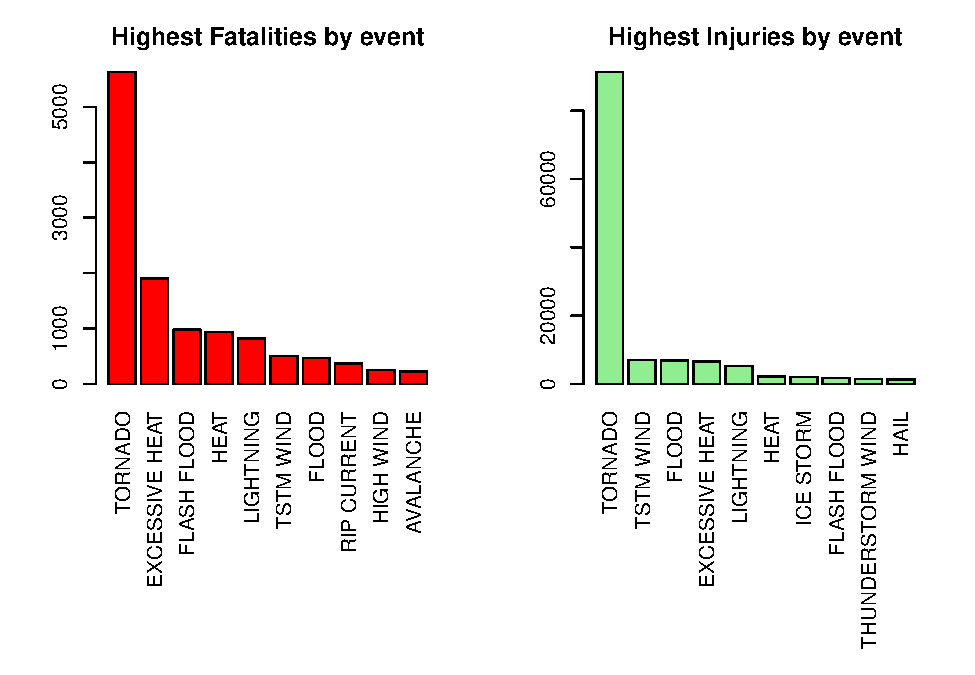
\includegraphics{rpubs-RR-project-2-_files/figure-latex/plothumanloss-1.pdf}

ploted top 10 events for high crop and property loss

\begin{Shaded}
\begin{Highlighting}[]
\KeywordTok{par}\NormalTok{(}\DataTypeTok{mfrow =} \KeywordTok{c}\NormalTok{(}\DecValTok{1}\NormalTok{, }\DecValTok{2}\NormalTok{), }\DataTypeTok{mar =} \KeywordTok{c}\NormalTok{(}\DecValTok{12}\NormalTok{, }\DecValTok{4}\NormalTok{, }\DecValTok{3}\NormalTok{, }\DecValTok{2}\NormalTok{), }\DataTypeTok{mgp =} \KeywordTok{c}\NormalTok{(}\DecValTok{3}\NormalTok{, }\DecValTok{1}\NormalTok{, }\DecValTok{0}\NormalTok{), }\DataTypeTok{cex =} \FloatTok{0.8}\NormalTok{)}
\KeywordTok{barplot}\NormalTok{(propdmg10}\OperatorTok{$}\NormalTok{PROPDMGCOST, }\DataTypeTok{las =} \DecValTok{3}\NormalTok{, }\DataTypeTok{names.arg =}\NormalTok{ propdmg10}\OperatorTok{$}\NormalTok{EVTYPE, }\DataTypeTok{main =} \StringTok{"Top 10 property loss by event"}\NormalTok{, }\DataTypeTok{col =} \StringTok{"light blue"}\NormalTok{)}
\KeywordTok{barplot}\NormalTok{(cropdmg10}\OperatorTok{$}\NormalTok{CROPDMGCOST, }\DataTypeTok{las =} \DecValTok{3}\NormalTok{, }\DataTypeTok{names.arg =}\NormalTok{ cropdmg10}\OperatorTok{$}\NormalTok{EVTYPE, }\DataTypeTok{main =} \StringTok{"Top 10 crop loss by event"}\NormalTok{, }\DataTypeTok{col =} \StringTok{"light blue"}\NormalTok{)}
\end{Highlighting}
\end{Shaded}

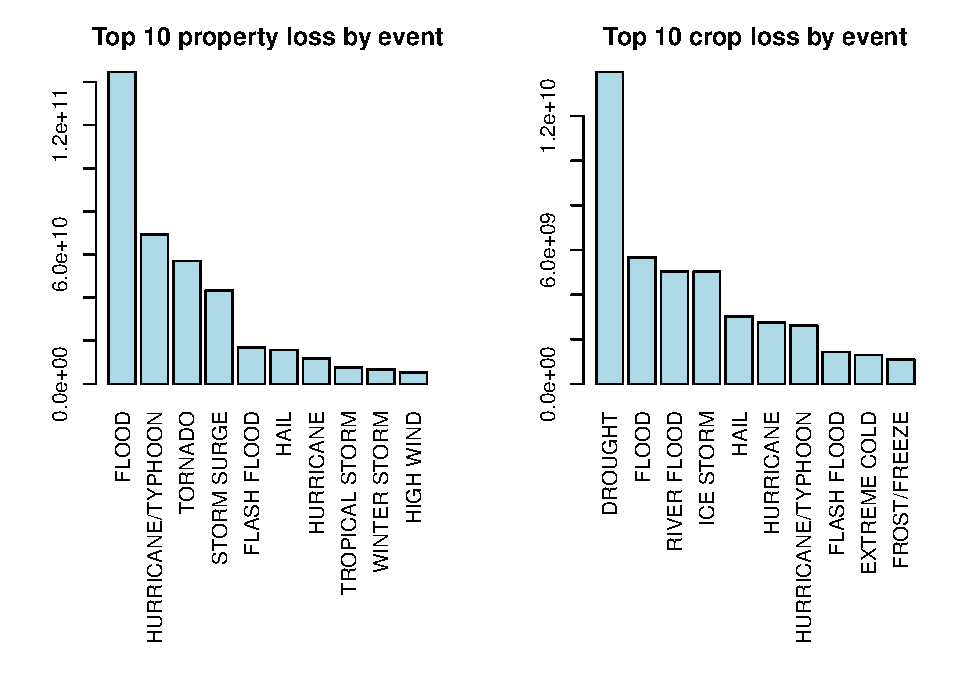
\includegraphics{rpubs-RR-project-2-_files/figure-latex/plotdmgloss-1.pdf}

\hypertarget{result}{%
\section{Result}\label{result}}

As per plot-1, there are highest fatalities and injuries due to Tornado.
Highest Property damage due to Floods and highest crop damage due to
Droughts

\end{document}
